\def\r{Pearson's r\xspace}
\def\ktau{Kendall's $\tau$\xspace}
\def\srho{Spearman's $\rho$\xspace}
\def\pb{Pointbiserial\xspace}
\def\student{Student's t-test\xspace}
\def\paired{Paired t-test\xspace}
\def\mannu{Mann-Whitney U\xspace}
\def\wilcox{Wilcoxon signed rank\xspace}
\def\welch{Welch's t-test\xspace}
\def\f{F-test\xspace}
\def\rm{Repeated measures one way ANOVA\xspace}
\def\kw{Kruskal Wallis\xspace}
\def\friedman{Friedman\xspace}
\def\facANOVA{Factorial ANOVA\xspace}
\def\twoANOVA{Two-way ANOVA\xspace}
\def\chiSq{Chi Square\xspace}
\def\fisher{Fisher's Exact\xspace}
\def\boot{Bootstrap\xspace}

\lstdefinestyle{teastyle}{
    backgroundcolor=\color{white},
    commentstyle=\color{codegreen},
    keywordstyle=\color{magenta},
    numberstyle=\tiny\color{codegray},
    stringstyle=\color{codepurple},
    basicstyle=\ttfamily\footnotesize,
    breakatwhitespace=false,
    breaklines=true,
    captionpos=b,
    keepspaces=true,
    numbers=left,
    numbersep=5pt,
    showspaces=false,
    showstringspaces=false,
    showtabs=false,
    tabsize=2,
    deletekeywords={input, print, id},
    % alsoletter={_},
    % literate={define_variables}{\textcolor{magenta}{define\_variables}}1,
    otherkeywords={tea.data, tea.define_variables, tea.define_study_design, tea.assume, tea.hypothesize}
    % here are the additional keywords
%     emph={data, define_variables, define_study_design, assume, hypothesize, <, >, =, !},
    % they are underlines
%     emphstyle={\textbf}
}

\newcommand{\figureTeaProgram}{
  % \lstset{deletekeywords={hypothesize}}
  \lstinputlisting[
        style=teastyle,
        % language=Python, 
        % keywordstyle=\color{black},  % choose your preferred color
        % morekeywords={},
        caption={\textbf{Sample Tea program.} 
        The specification outlines an observational study to analyze the relationship between geographic location (`So') and probability of imprisonment (`Prob') in a common USCrime data set~\protect\cite{venables2013modern,kabacoff2011action}. 
        See~\autoref{usageScenarioTea} for an explanation of the code. Tea programs specify 1) data, 2) variables, 3) study design, 4) assumptions, and 5) hypotheses.
        % \end{small}
        },
        label={lst:tea_program}
  ]{tea/figures/tea-example.py}

  % \renewcommand{\theFancyVerbLine}{
  % \sffamily\textcolor[rgb]{0.5,0.5,0.5}{\scriptsize\arabic{FancyVerbLine}}}

  % \begin{minted}[mathescape,
  %               linenos,
  %               numbersep=5pt,
  %               gobble=2,
  %               frame=lines,
  %               framesep=2mm]{csharp}
  %   string title = "This is a Unicode π in the sky"
  %   /*
  %   Defined as $\pi=\lim_{n\to\infty}\frac{P_n}{d}$ where $P$ is the perimeter
  %   of an $n$-sided regular polygon circumscribing a
  %   circle of diameter $d$.
  %   */
  %   const double pi = 3.1415926535
  % \end{minted}


% \begin{figure}
%     % \vspace{-5pt}
%     \centering
%     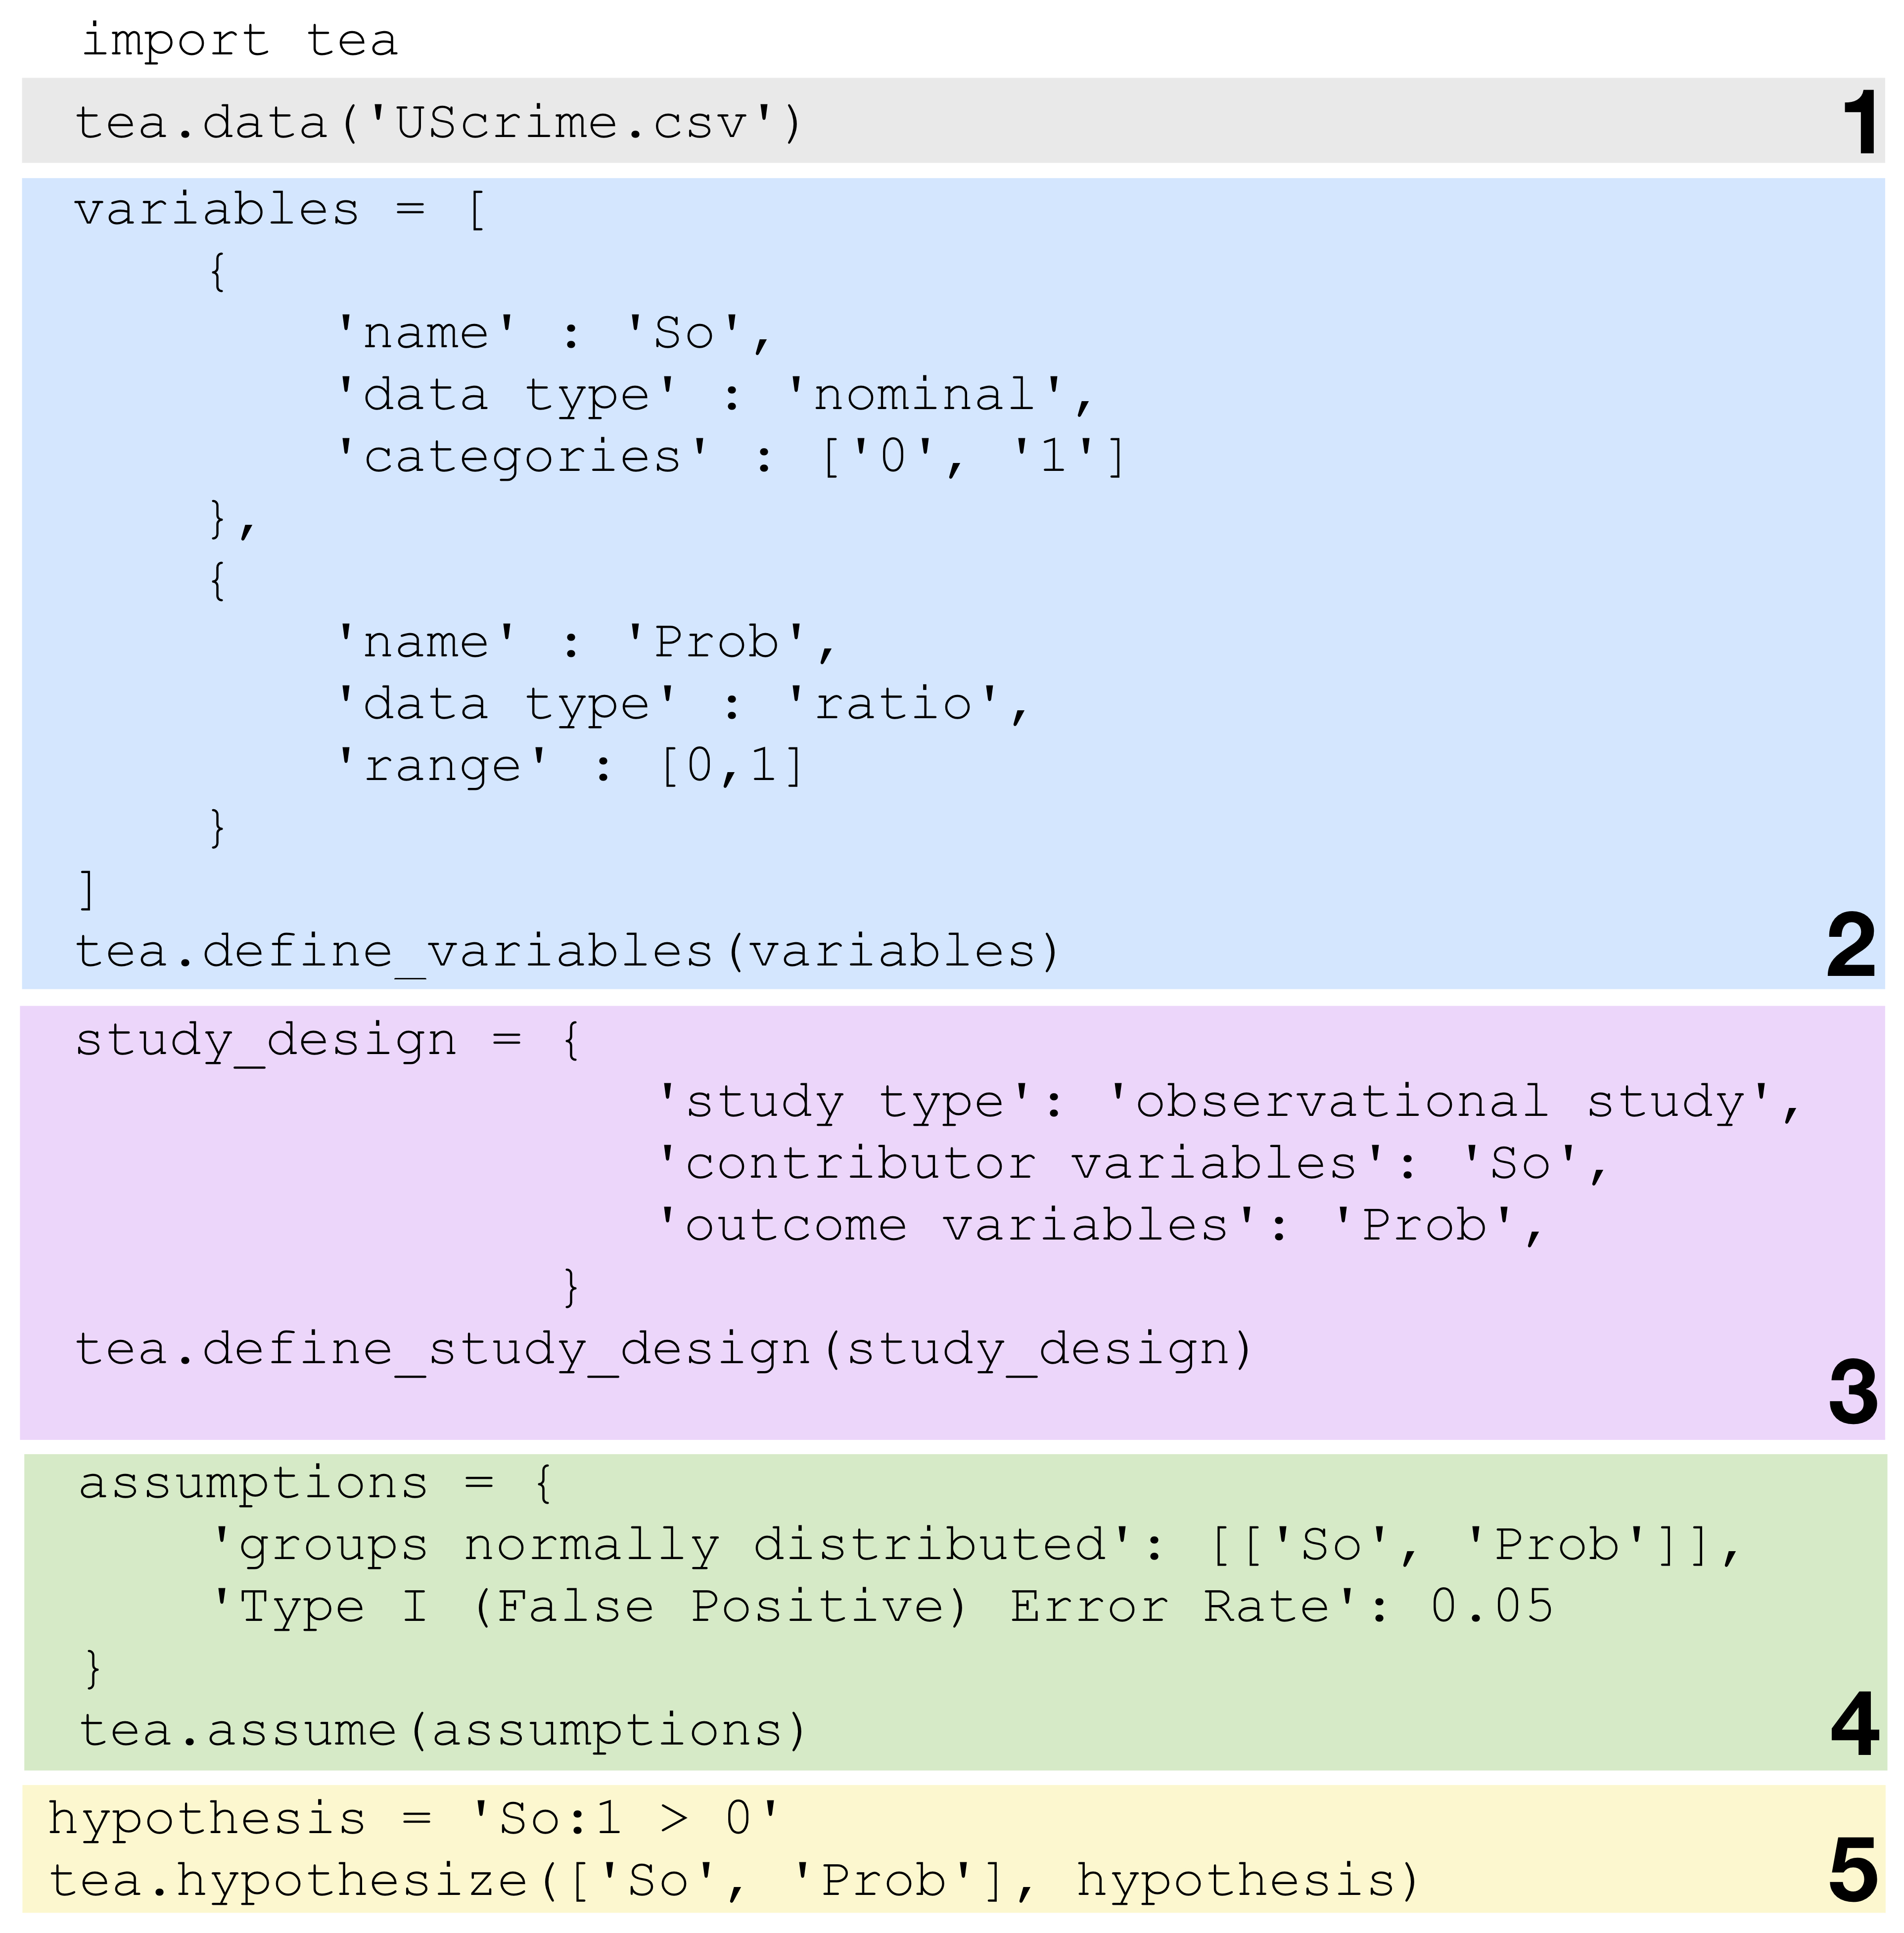
\includegraphics[width=0.5\columnwidth, clip]{tea/figures/tea_program.jpg}
%     % \vspace{-15pt} 
%     \caption{\textbf{Sample Tea program.}}
%       \begin{small}
%       \begin{minipage}{\linewidth}
%         The specification outlines an experiment to analyze the relationship between geographic location (`So') and probability of imprisonment (`Prob') in a common USCrime data set~\protect\cite{venables2013modern,kabacoff2011action}.
%         See~\autoref{usageScenarioTea} for an explanation of the code. Tea programs specify 1) data, 2) variables, 3) study design, 4) assumptions, and 5) hypotheses.
%       \end{minipage}
%       \end{small} 
%     \label{lst:tea_program}
%     \vspace{-\baselineskip}
% \end{figure}
}


\def\r{Pearson's r}
\def\ktau{Kendall's $\tau$}
\def\srho{Spearman's $\rho$}
\def\pb{Pointbiserial}
\def\student{Student's t-test}
\def\paired{Paired t-test}
\def\mannu{Mann-Whitney U}
\def\wilcox{Wilcoxon signed rank}
\def\welch{Welch's}
\def\f{F-test}
\def\rm{Repeated measures one way ANOVA}
\def\kw{Kruskal Wallis}
\def\friedman{Friedman}
\def\facANOVA{Factorial ANOVA}
\def\twoANOVA{Two-way ANOVA}
\def\chiSq{Chi Square}
\def\fisher{Fisher's Exact}

\newcommand{\tableTeaTests}{
    \begin{table*}[htbp]
      \begin{center} \singlespacing
      \caption{Statistical tests supported in Tea's Null Hypothesis Significance Testing module} \label{tab:tea_tests}
      \begin{tabular}{lll}
      \toprule
      \colH{Class of tests}           & \colH{Parametric} & \colH{Non-parametric} \\
        Correlation                   & \r                &  \ktau   \\
                                      & \pb               &  \srho  \\
        \midrule
        Bivariate mean comparison     & \student          & \welch \\
                                      &                   & \mannu \\
                                      &                   & (a.k.a. Wilcoxon rank sum) \\
                                      & \paired           & \wilcox \\
        \midrule
        Multivariate mean comparison  & \f                & \kw   \\
                                      & \rm               & \friedman \\
                                      & \twoANOVA         & \\
                                      & \facANOVA         & \\
        \midrule
        \midrule
        Proportions: \chiSq , \fisher and Others: Bootstrapping (with confidence intervals) \\
      \bottomrule
      \end{tabular}
      \end{center}
    \end{table*}
}

\newcommand{\furtherTestResults}{
\begin{table*}[htbp]
  \begin{center}
    \caption{Results from Factorial ANOVA for RM ANOVA example.}
    \begin{tabularx}{\linewidth}{XXXXXX}
       & \textbf{df} & \textbf{sum\_sq} & \textbf{mean\_sq} & \textbf{F} & \textbf{PR(>F)} \\
      C(conc) & 6.0 & 4068.771429 & 678.128571 & 9.261087 & 1.242777e-07 \\
      Residual & 77.0 & 5638.204167  & 73.223431   &    NaN     &      NaN \\
    \end{tabularx}
    \end{center}
    \label{tab:rm_anova_fanova}
\end{table*}

\begin{table*}[htpb]
  \begin{center}
    \caption{Results from F test for F test example.}
    \begin{tabularx}{\linewidth}{XXXXXX}
       & \textbf{df} & \textbf{sum\_sq} & \textbf{mean\_sq} & \textbf{F} & \textbf{PR(>F)} \\
        C(trt)   &  4.0 & 1351.369014 & 337.842253 & 32.432826 & 9.818516e-13 \\
        Residual & 45.0 &  468.750438  & 10.416676    &    NaN       &    NaN \\
    \end{tabularx}
  \end{center}
  \label{tab:f_test_f_test}
\end{table*}

\begin{table*}[htpb]
  \begin{center}
    \caption{Results from Factorial ANOVA test for F test example.}
    \begin{tabularx}{\linewidth}{XXXXXX}
       & \textbf{df} & \textbf{sum\_sq} & \textbf{mean\_sq} & \textbf{F} & \textbf{PR(>F)} \\
        C(trt)   &  4.0 & 1351.369014 & 337.842253 & 32.432826 & 9.818516e-13 \\
        Residual & 45.0 &  468.750438  & 10.416676    &    NaN       &    NaN \\
    \end{tabularx}
  \end{center}
  \label{tab:f_test_fanova}
\end{table*}

\begin{table*}[htpb]
  \begin{center}
    \caption{Results from Factorial ANOVA test for Paired T test example.}
    \begin{tabularx}{\linewidth}{XXXXXX}
       & \textbf{df} & \textbf{sum\_sq} & \textbf{mean\_sq} & \textbf{F} & \textbf{PR(>F)} \\
        C(Group) &  1.0 &  294.0  &  294.0 & 2.826923 & 0.106839 \\
        Residual & 22.0 & 2288.0  &  104.0    &   NaN   &    NaN \\
    \end{tabularx}
  \end{center}
  \label{tab:paired_t_fanova}
\end{table*}


\begin{table*}[htpb]
  \begin{center}
    \caption{Results from F test and Factorial ANOVA for Student's T test example.}
    \begin{tabularx}{\linewidth}{XXXXXX}
       & \textbf{df} & \textbf{sum\_sq} & \textbf{mean\_sq} & \textbf{F} & \textbf{PR(>F)} \\
        C(So)   &   1.0 &  0.006702 &  0.006702 & 17.657903 & 0.000124 \\
        Residual & 45.0 & 0.017079 & 0.000380    &    NaN     &  NaN \\
    \end{tabularx}
  \end{center}
  \label{tab:students_t_f_test_and_fanova}
\end{table*}
}

\begin{comment}
% make a custom style that looks good and can highlight some additional keywords
\lstdefinestyle{tea}{
  basicstyle=\ttfamily,
  deletekeywords={input, print, id},
  language=Python,
  % here are the additional keywords
  emph={data, define_variables, define_study_design, assume, hypothesize, <, >, =, !},
  % they are underlines
  emphstyle={\bf},
}
\lstset{
  % use this style by default
  style=tea,
  % look better
  columns=flexible,
  showstringspaces=false,
  % spacing, size, numbers, etc.
  numbers=left,
  xleftmargin=2em,
  numberstyle=\tiny,
  escapechar=|,
}
\end{comment}

\newcommand{\teaHypotheses}{
  \begin{figure}[t]
    \vspace{-5pt}
    \centering
    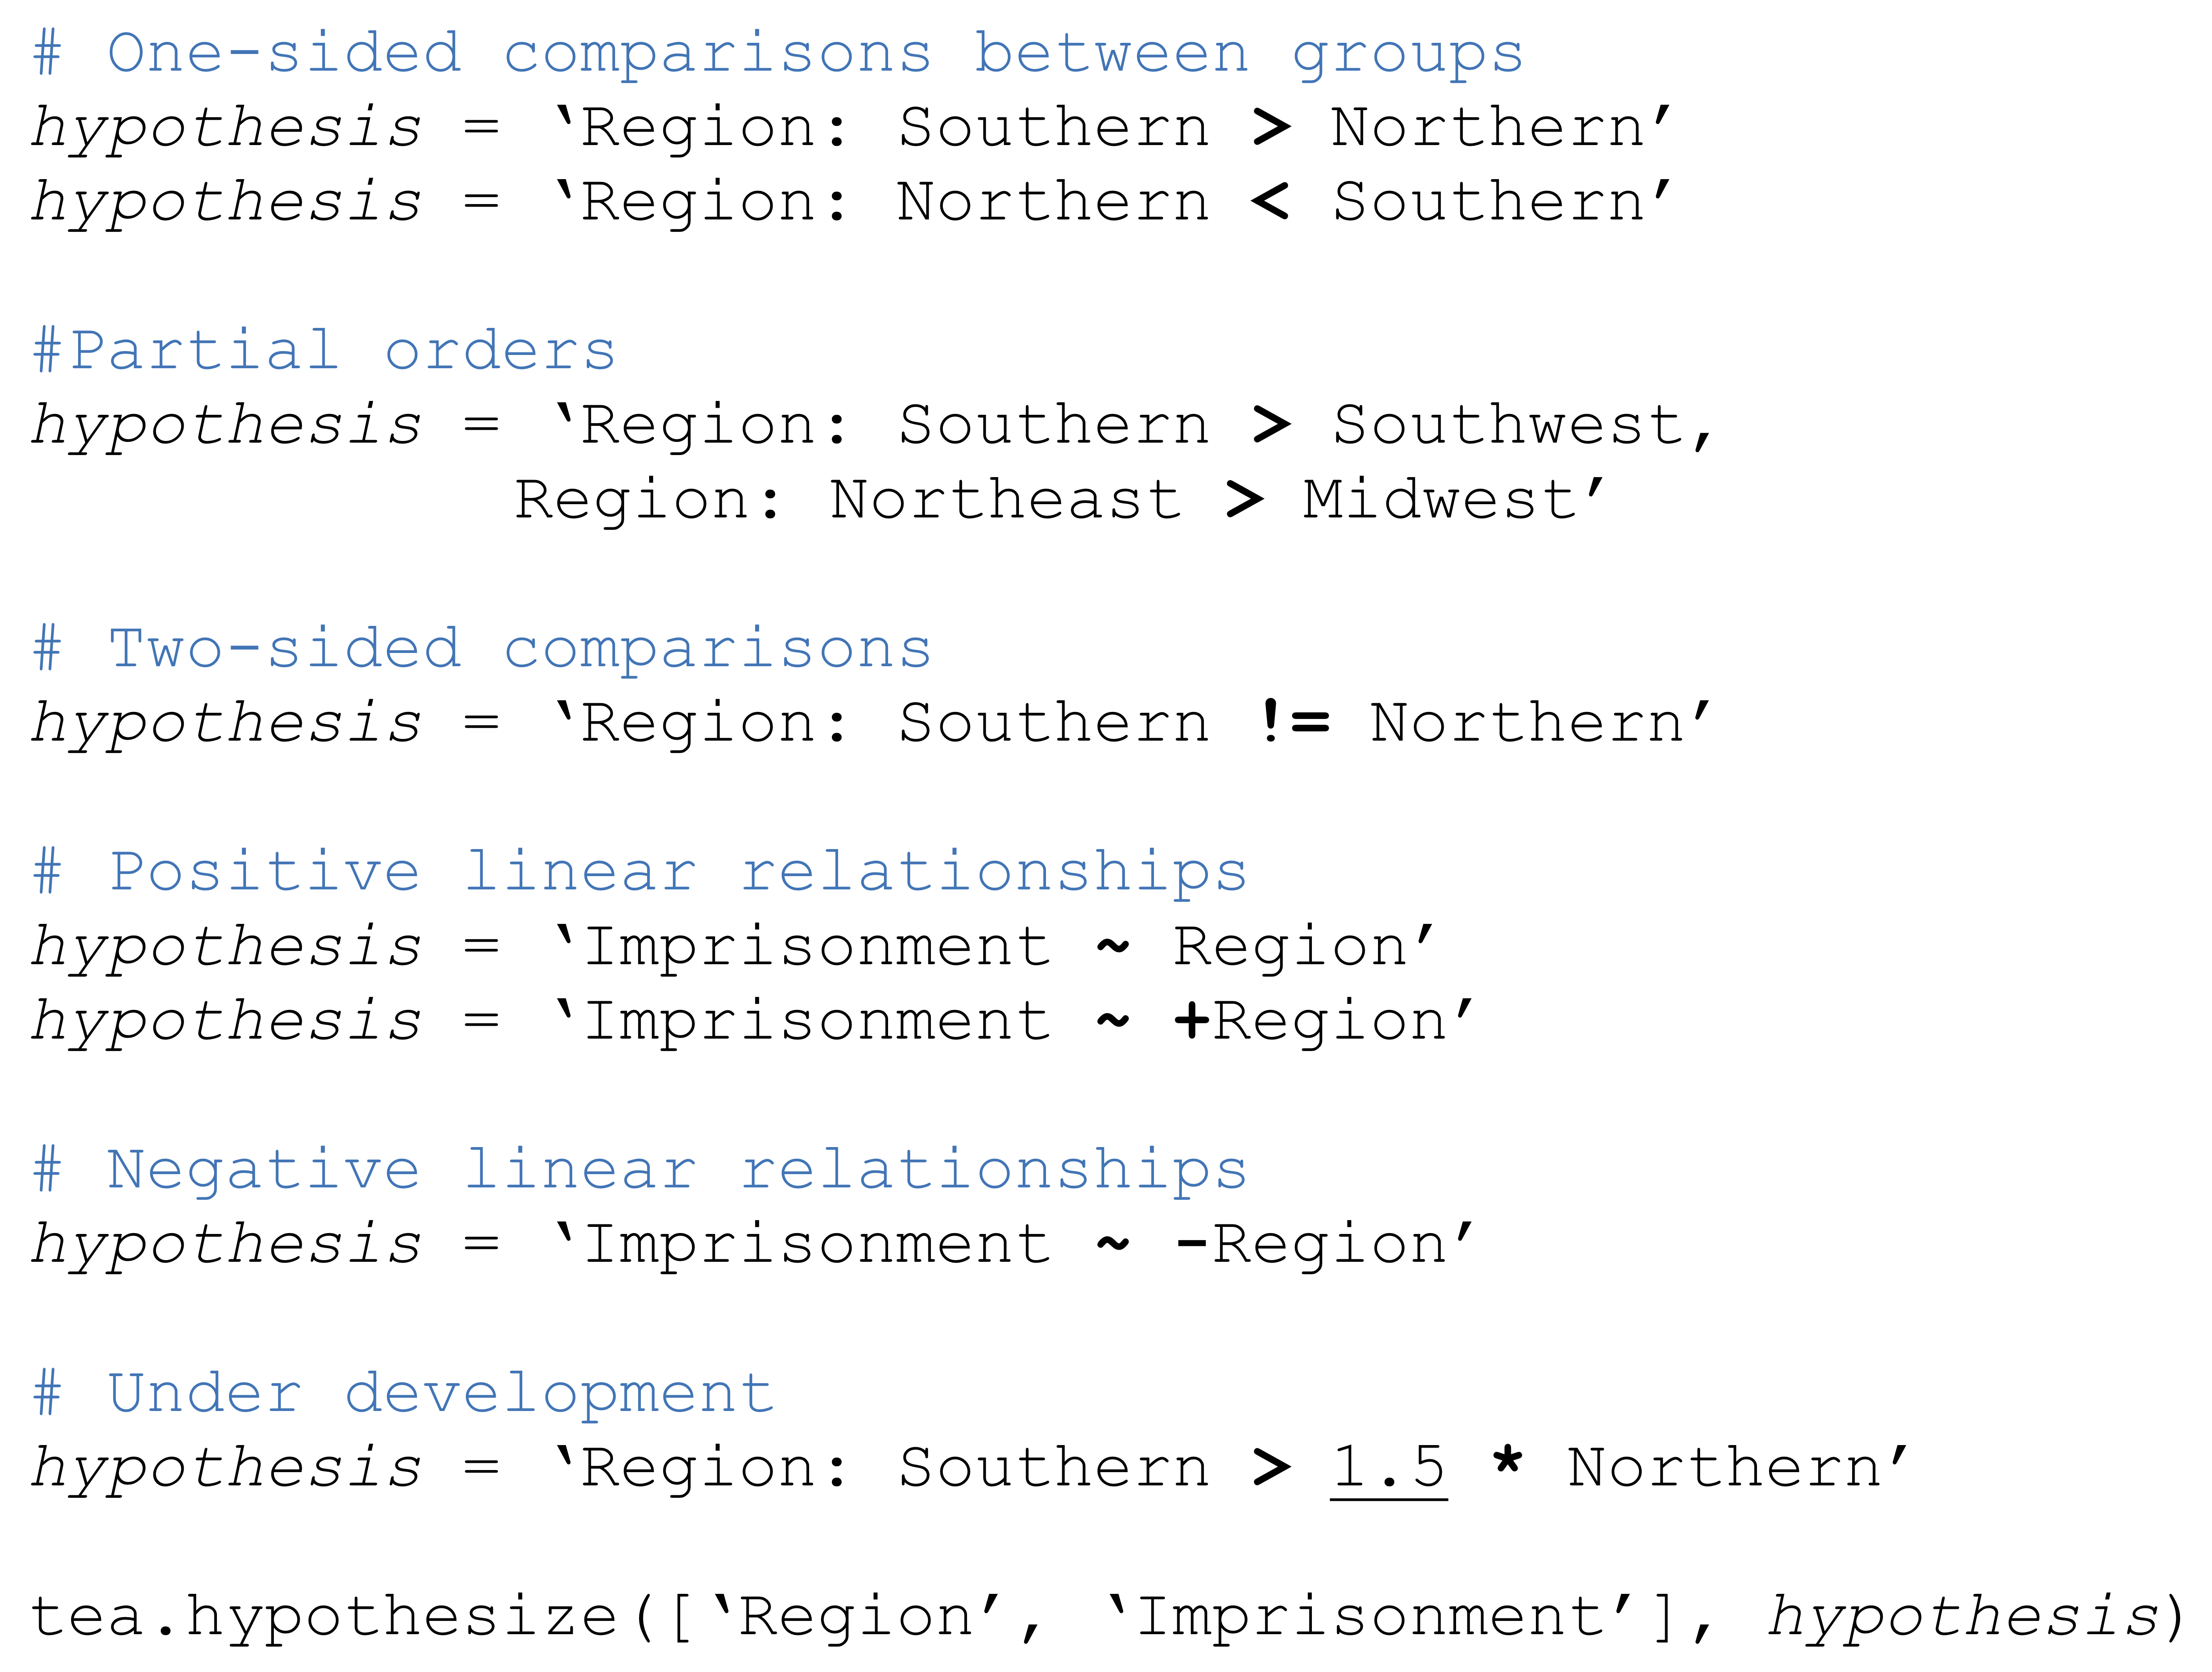
\includegraphics[width=1.\columnwidth, clip]{tea/figures/tea_hypotheses.png}
    % \vspace{-15pt}
    \caption{\textbf{Hypotheses that users can express in Tea.} }
    \label{fig:teaHypotheses}
    \vspace{-\baselineskip}
    \vspace{-3pt}
  \end{figure}
}


\newcommand{\otherSystems}{
    \begin{table*}[t]
        \centering \small
        \caption{\textbf{Comparison of Tea to other tools.}}
          \begin{small}
          \begin{minipage}{\linewidth}
            Despite the published best practices for statistical analyses, most
            tools do not help users select appropriate tests. Tea not only
            addresses the best practices but also supports reproducing analyses.
            Below, $\sim$ indicates a practice is sometimes supported.
          \end{minipage}
          \end{small}
        \label{tab:otherSystems}
        \begin{tabularx}{\linewidth}{r|c|c|c|c|c|c}
          \toprule
            \colHR{Best practices} & \colH{SAS} & \colH{SPSS} & \colH{JMP} & \colH{R} & \colH{\makecell{Statsplorer\\\cite{wacharamanotham2015statsplorer}}} & \colH{Tea} \\
            \midrule \\ 
            % & & & & & \colH{\cite{wacharamanotham2015statsplorer}} & \\
            % \midrule \\ 
            Explicit statement of user assumptions & \no & \no & \no & \no & \no & \yes \\
            Automatic verification of test preconditions & \no & \no & $\sim$ & $\sim$ & \yes & \yes \\
            Automatic accounting of multiple comparisons & \no & \no & \no & \no & \yes & \yes \\
            Surface alternative analyses & \no & \no & \no & \no & \no & \yes \\
            Contextualize results & \yes & $\sim$ & \yes & $\sim$ & \yes & \yes \\
            Easy to reproduce analysis & \yes & \yes & \no & \yes & \no & \yes \\
        \end{tabularx}
    \end{table*}
}


\newcommand{\figureOutputTTest}{
  \begin{figure}[t]
    \vspace{-15pt}
    % \centering
    \fbox{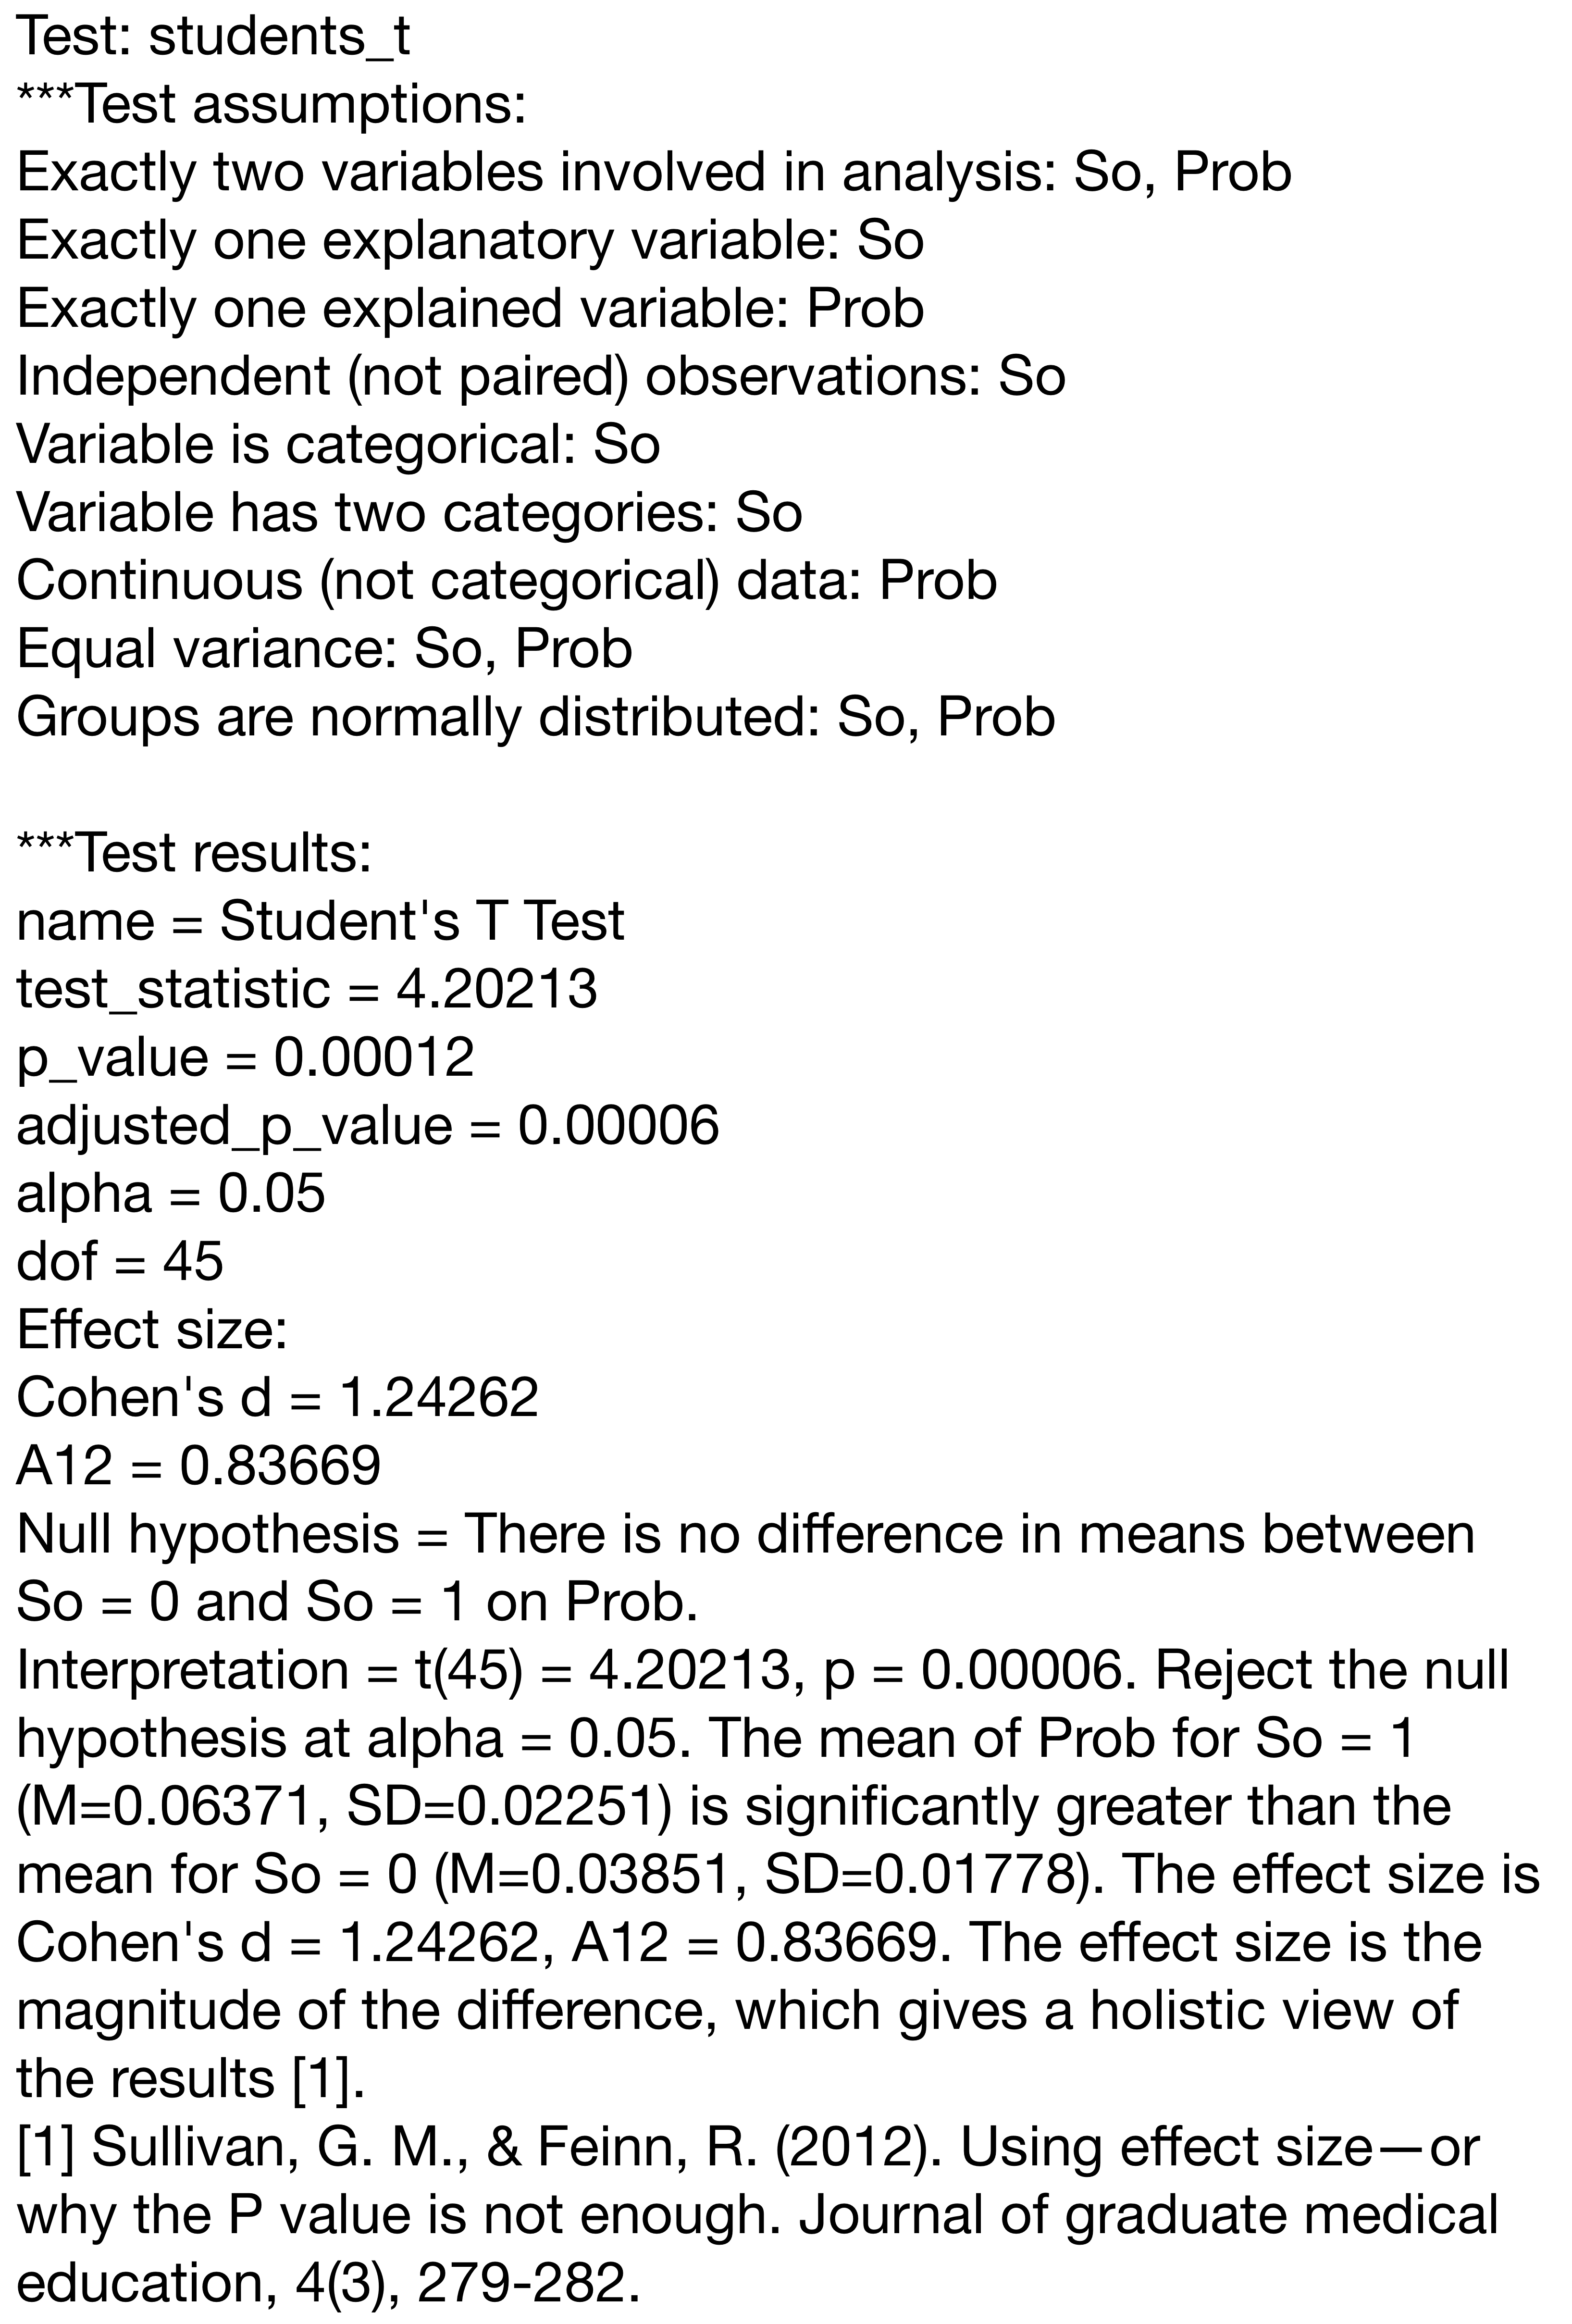
\includegraphics[width=.8\columnwidth, clip]{tea/figures/tea_output_t_test.jpg}}
    \vspace{2pt}
    \caption{\textbf{Part of Tea's output.} The output is a result of running the sample program in \autoref{lst:tea_program}. Tea outputs the data properties that led Tea to select the statistical test as well as results from executing the test, effect size calculations, the null hypothesis tested, and the interpretation of the results, which can be included in publications with minor editing.}
    \label{fig:output_t_test}
    \vspace*{-\baselineskip}
    \vspace{-15pt}
  \end{figure}
}

\newcommand{\figureModes}{
  \begin{figure}[H]
    % \vspace{-5pt}
    \centering
    \includegraphics[width=\textwidth]{tea/figures/modes_wide.jpg}
    \vspace{-10pt}
    \caption{\textbf{Tea program and its mode-dependent executions.}}
      \begin{small}
      \begin{minipage}{\linewidth}
        a) Tea program that aims to determine if two contributor variables, `Illiteracy` and `HS Grad' that may predict a third outcome variable `Life Exp', are correlated. The user asserts that `Illiteracy' is normally distributed. 
        b) By default, Tea executes programs in the \textit{strict} mode. 
        c) Warning that Tea disagrees with the user and will override the user's assertion that `Illiteracy' is normally distributed in the \textit{strict} mode. 
        d) Results without the parametric test since Tea overrides user's assertion. 
        e) A single line change can modify Tea to execute a program in \textit{relaxed} mode. 
        f) Warning that Tea cannot verify normality for `Illiteracy' but will defer to user's assertion. 
        g) Results with the parametric test since Tea proceeds as if  `Illiteracy' was normally distributed.
      \end{minipage}
      \end{small}
    \label{fig:modes}
    \vspace*{-\baselineskip}
  \end{figure}
}
 
\newcommand{\figureSyntacticSugar}{
  \begin{figure}
      \centering
      \subcaptionbox{Specify the test.}
      {\fbox{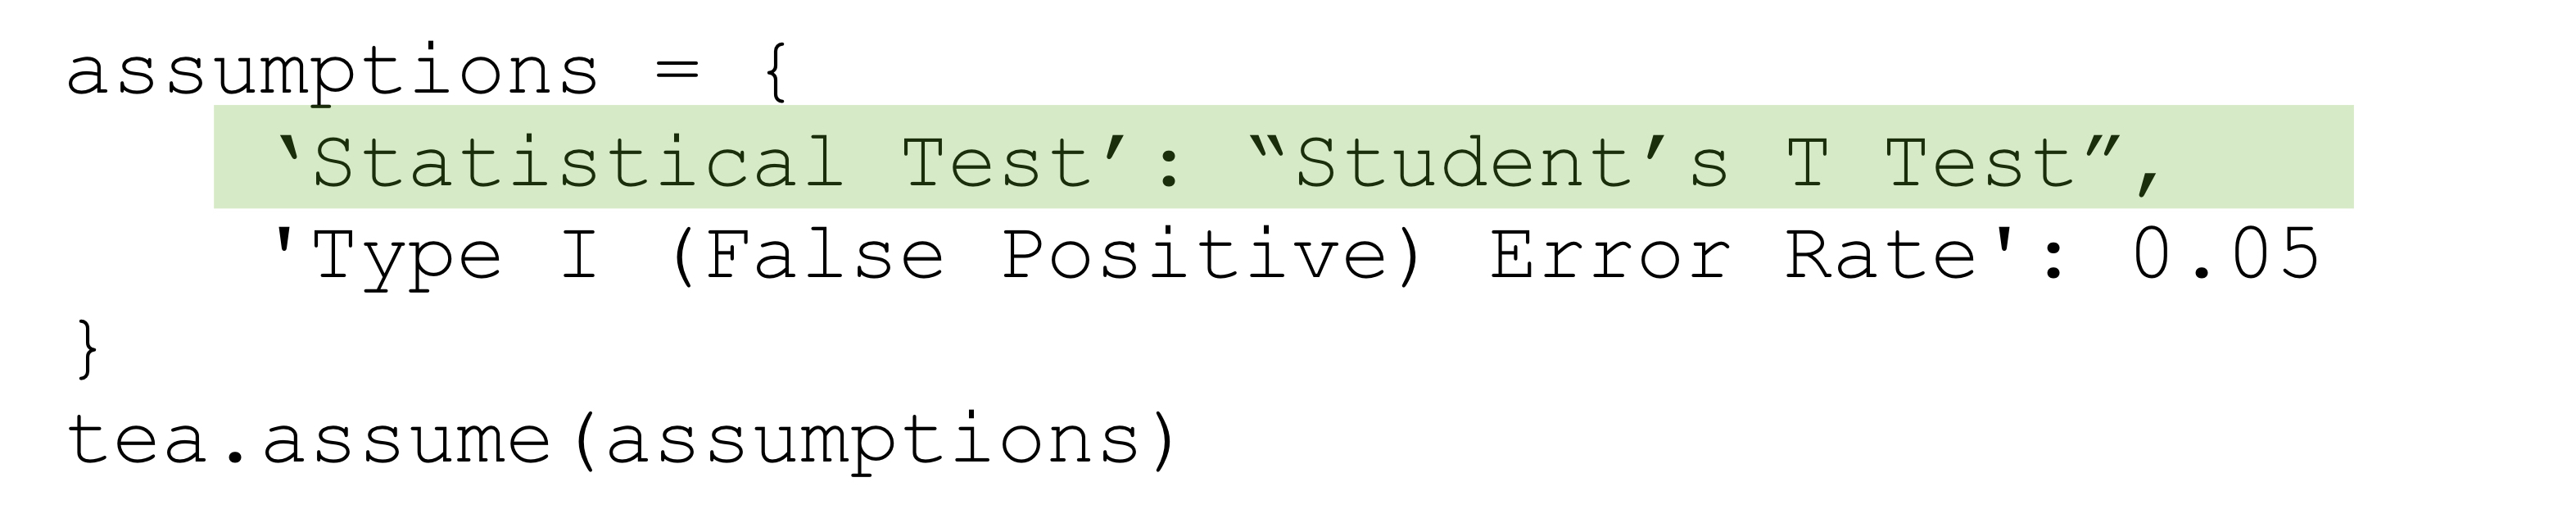
\includegraphics[width=\linewidth, clip]{tea/figures/sugar_test.jpg}}}
      \label{fig:sugar_expanded}
      \subcaptionbox{Specify the properties.}
      {\fbox{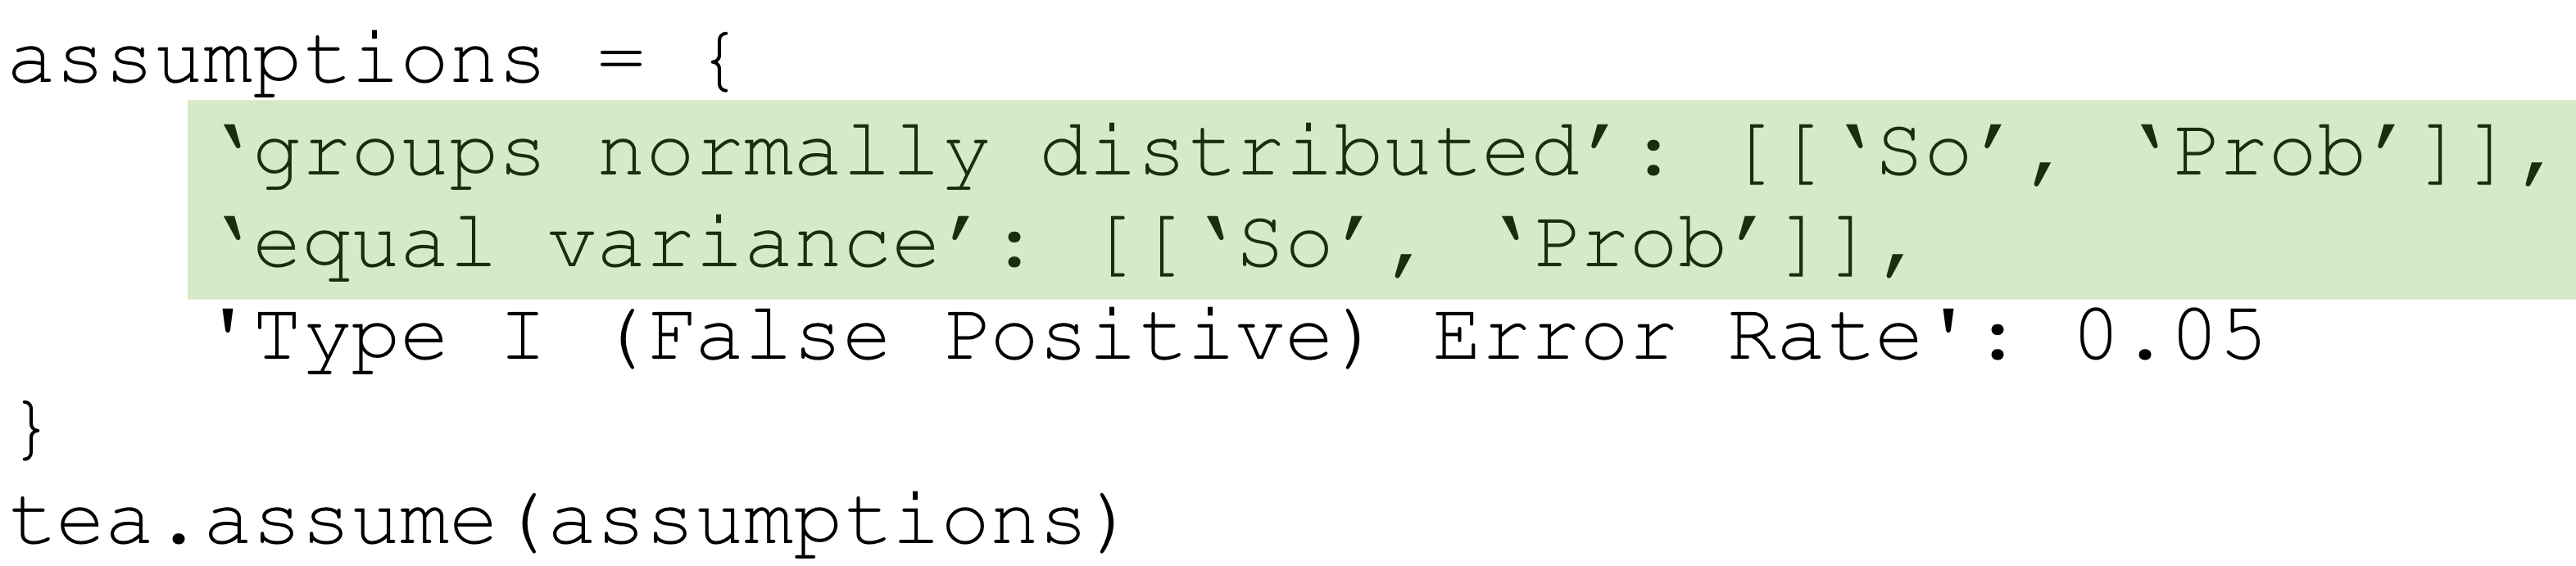
\includegraphics[width=\linewidth, clip]{tea/figures/sugar_expanded.jpg}}}
      \label{fig:sugar_test}
      % \vspace{-10pt}
    \caption{\textbf{Tea can support pre-registration.} Tea programs provide an executable format for pre-registration. When pre-registering studies, users can explicitly state their assumptions about data properties or specify the exact statistical test they intend to run with data. Specifying the name of a test (a) is \textit{syntactic sugar} for the more verbose form (b). The above code snippets are semantically equivalent.}
    \label{fig:sugar}  
    \vspace*{-\baselineskip}
    % \vspace{-3pt}
    \end{figure}
}
